\documentclass[tikz,border=2mm]{standalone}
\usepackage{amsmath}
\usepackage{helvet}
\renewcommand{\familydefault}{\sfdefault}
\usetikzlibrary{arrows.meta,calc,positioning}

\definecolor{charcoal}{RGB}{40,48,54}
\definecolor{grayline}{RGB}{112,124,132}
\definecolor{sulfur}{RGB}{239,190,49}
\definecolor{warm}{RGB}{207,77,55}
\definecolor{cool}{RGB}{48,112,151}
\definecolor{wash}{RGB}{246,247,246}

\begin{document}
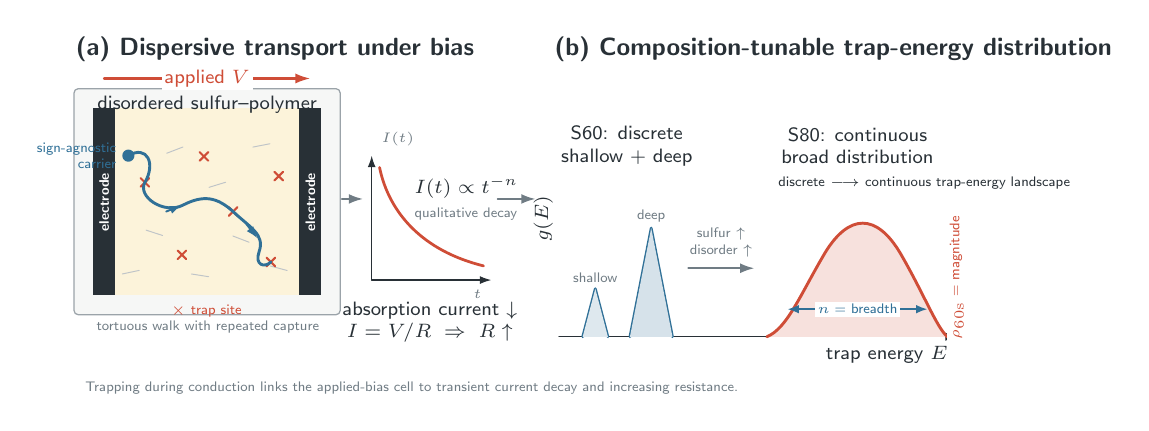
\begin{tikzpicture}[
  x=1cm,y=1cm,
  line cap=round,line join=round,
  >={Latex[length=1.8mm,width=1.25mm]},
  txt/.style={font=\scriptsize,text=charcoal},
  note/.style={font=\tiny,text=grayline},
  arrow/.style={-{Latex[length=1.8mm,width=1.25mm]},draw=grayline,line width=.65pt},
  trap/.style={draw=warm,line width=.75pt}
]

% headings
\node[anchor=west,font=\small\bfseries,text=charcoal] at (0,4.55)
  {(a) Dispersive transport under bias};
\node[anchor=west,font=\small\bfseries,text=charcoal] at (6.08,4.55)
  {(b) Composition-tunable trap-energy distribution};

% PANEL A: compact cell
\draw[rounded corners=1.5pt,draw=grayline!70,fill=wash,line width=.45pt]
  (.10,1.18) rectangle (3.48,4.05);
\fill[charcoal] (.34,1.43) rectangle (.62,3.80);
\fill[charcoal] (2.96,1.43) rectangle (3.24,3.80);
\fill[sulfur!18] (.62,1.43) rectangle (2.96,3.80);
\node[rotate=90,font=\tiny\bfseries,text=white] at (.48,2.61) {electrode};
\node[rotate=90,font=\tiny\bfseries,text=white] at (3.10,2.61) {electrode};
\node[txt,anchor=south] at (1.79,3.62) {disordered sulfur--polymer};

% applied voltage without electrode polarity assignment
\draw[draw=warm,line width=.75pt,-{Latex[length=1.9mm,width=1.3mm]}]
  (.48,4.18)--(3.10,4.18);
\node[txt,text=warm,fill=white,inner sep=1pt] at (1.79,4.18) {applied $V$};

% amorphous texture
\foreach \x/\y/\r in {
 .82/1.72/12,1.12/2.22/-18,1.38/3.27/21,1.70/1.68/-9,
 1.92/2.83/17,2.22/2.14/-21,2.48/3.33/11,2.70/1.77/-15}
  \draw[grayline!45,line width=.35pt,rotate around={\r:(\x,\y)}]
    (\x-.11,\y)--(\x+.11,\y);

% chemically agnostic trap marks
\foreach \x/\y in {1.00/2.86,1.47/1.94,1.75/3.19,2.12/2.49,2.60/1.85,2.70/2.94}{
  \draw[trap] (\x-.055,\y-.055)--(\x+.055,\y+.055)
              (\x-.055,\y+.055)--(\x+.055,\y-.055);
}

% sign-agnostic, non-ballistic repeated-trapping trajectory
\draw[cool,line width=1.05pt]
  (.79,3.20)
  .. controls (1.03,3.34) and (1.14,3.10) .. (1.00,2.86)
  .. controls (.90,2.68) and (1.24,2.45) .. (1.48,2.57)
  .. controls (1.75,2.71) and (1.92,2.67) .. (2.12,2.49)
  .. controls (2.33,2.29) and (2.53,2.20) .. (2.45,1.98)
  .. controls (2.39,1.81) and (2.52,1.77) .. (2.60,1.85);
\draw[cool,line width=.7pt,-{Latex[length=1.55mm,width=1.05mm]}]
  (1.27,2.49)--(1.47,2.57);
\draw[cool,line width=.7pt,-{Latex[length=1.55mm,width=1.05mm]}]
  (2.29,2.33)--(2.43,2.15);
\fill[cool] (.79,3.20) circle (2.2pt);
\node[note,text=cool,anchor=east,align=right] at (.76,3.20)
  {sign-agnostic\\carrier};
\node[note,text=warm,anchor=north] at (1.78,1.43) {$\times$ trap site};
\node[note,align=center] at (1.80,1.02) {tortuous walk with repeated capture};

% transition from cell to qualitative transient current
\draw[arrow] (3.50,2.65)--(3.77,2.65);
\begin{scope}[shift={(3.88,1.62)}]
  \draw[draw=charcoal,line width=.45pt,-{Latex[length=1.45mm,width=1mm]}]
    (0,0)--(1.52,0) node[note,below left] {$t$};
  \draw[draw=charcoal,line width=.45pt,-{Latex[length=1.45mm,width=1mm]}]
    (0,0)--(0,1.58) node[note,above right] {$I(t)$};
  \draw[draw=warm,line width=1pt]
    (.10,1.43) .. controls (.22,.85) and (.65,.37) .. (1.42,.18);
  \node[txt,anchor=west] at (.42,1.18) {$I(t)\propto t^{-n}$};
  \node[note,anchor=west] at (.42,.84) {qualitative decay};
\end{scope}
\node[txt,align=center] at (4.62,1.08)
  {absorption current $\downarrow$\\$I=V/R\;\Rightarrow\;R\uparrow$};

% bridge into the energy-distribution explanation
\draw[arrow] (5.48,2.65)--(5.96,2.65);

% PANEL B: distributions share an energy baseline
\begin{scope}[shift={(6.14,.55)}]
  \draw[draw=charcoal,line width=.5pt,-{Latex[length=1.55mm,width=1.05mm]}]
    (.12,.35)--(5.18,.35) node[txt,below left] {trap energy $E$};
  \node[txt,rotate=90] at (-.08,1.85) {$g(E)$};

  % Low-sulfur discrete shallow and deep states
  \draw[cool,line width=1pt]
    (.42,.35)--(.58,.96)--(.74,.35)
    (1.02,.35)--(1.29,1.73)--(1.56,.35);
  \fill[cool!16] (.42,.35)--(.58,.96)--(.74,.35)--cycle;
  \fill[cool!20] (1.02,.35)--(1.29,1.73)--(1.56,.35)--cycle;
  \node[txt,align=center] at (.98,2.77)
    {S60: discrete\\shallow + deep};
  \node[note] at (.58,1.10) {shallow};
  \node[note] at (1.29,1.88) {deep};

  % Increasing sulfur/disorder
  \draw[arrow] (1.76,1.22)--(2.60,1.22);
  \node[note,align=center] at (2.18,1.55) {sulfur $\uparrow$\\disorder $\uparrow$};

  % High-sulfur continuous broad landscape
  \path[fill=warm!17]
    (2.76,.35)
    .. controls (3.02,.46) and (3.18,.88) .. (3.50,1.42)
    .. controls (3.80,1.91) and (4.15,1.93) .. (4.46,1.40)
    .. controls (4.76,.88) and (4.91,.48) .. (5.05,.35)--cycle;
  \draw[warm,line width=1.05pt]
    (2.76,.35)
    .. controls (3.02,.46) and (3.18,.88) .. (3.50,1.42)
    .. controls (3.80,1.91) and (4.15,1.93) .. (4.46,1.40)
    .. controls (4.76,.88) and (4.91,.48) .. (5.05,.35);
  \node[txt,align=center] at (3.91,2.77)
    {S80: continuous\\broad distribution};

  % Orthogonal encodings: breadth versus magnitude
  \draw[cool,line width=.7pt,{Latex[length=1.45mm]}-{Latex[length=1.45mm]}]
    (3.02,.70)--(4.80,.70);
  \node[note,text=cool,fill=white,inner sep=1pt] at (3.91,.70)
    {$n$ = breadth};
  \draw[warm,line width=.7pt,{Latex[length=1.45mm]}-{Latex[length=1.45mm]}]
    (5.17,.38)--(5.17,1.83);
  \node[note,text=warm,rotate=90,fill=white,inner sep=1pt] at (5.17,1.10)
    {$\rho_{60\mathrm{s}}$ = magnitude};

  \node[note,text=charcoal,anchor=west] at (2.78,2.30)
    {discrete $\longrightarrow$ continuous trap-energy landscape};
\end{scope}

% concise causal statement
\node[note,text=grayline,anchor=west] at (.12,.25)
  {Trapping during conduction links the applied-bias cell to transient current decay and increasing resistance.};

\end{tikzpicture}
\end{document}
